\documentclass{asaproc}

\usepackage{dsfont}
\usepackage{graphicx}
\usepackage{bm}
\newcommand{\m}[1]{\mathbf{\bm{#1}}}
\newcommand{\R}{I\hspace{-4.4pt}R}

%\usepackage{times}
%If you have times installed on your system, please
%uncomment the line above

%For figures and tables to stretch across two columns
%use \begin{figure*} \end{figure*} and
%\begin{table*}\end{table*}
% please place figures & tables as close as possible
% to text references


\newcommand{\be}{\begin{equation}}
\newcommand{\ee}{\end{equation}}

\title{UK voter preferences on the EU referendum}

%input all authors' names

\author{Mickey Warner \\ AMS 207 Quiz 2}

%input affiliations

%{USDA Forest Service Forest Products Laboratory}

\begin{document}

\maketitle


\begin{abstract}
On 23 June 2016, the United Kingdom will hold a referendum to decide whether the nation should leave or remain in the European Union. Beginning September 2015, a variety of online and phone polls have been conducted to measure public preference on the issue. We consider regression models with linear time trends and additive effects for the polling source and for the type of poll (online or phone). We find evidence supporting a time trend with small effects due to the sources and the type of poll.
\end{abstract}

\section{Introduction}

Leading up to the 23 June 2016 referendum, over the course of nine months, starting September 2015, nine sources have published a total of one hundred polling results. The polls inquired voter preference on whether the United Kingdom (UK) should leave or remain in the European Union (EU). The possible choices for the respondents were ``leave'', ``remain'', and ``don't know.'' We will be interested in the proportion of people who prefer to leave given that an opinion was given (i.e., we ignore the ``don't know'' group).

Respondents giving ``don't know'' as their preference accounted for about 16\% of the voters in each poll (on average). Such a response may provide some information for preference on the referendum, but when it comes to voting time, a vote of ``I don't know'' will not contribute to a decision.

The surveys came in two forms, either online or by phone. The majority of polls were online (78\%) while the the rest were phone (22\%). Most sources were favored one kind of poll over the other. Only one source (Survation) had roughly half online (6 of 10) and half phone (4 of 10). Two other sources (ComRes and ICM) provided surveys of both types, but ComRes only 1 of 10 polls online and ICM had 35 of 37 online. The remainder of the sources provided only one type of poll.

A few of the sources published very few polls: BMG did 5, Opinium did 3, and Panelbase did 1 (all online). These three sources were combined into the Other category. By combining them, we are assuming they each provide the same effect on the outcome of the polls (i.e. their methodology is biased in the same way). This assumption may not be valid, but it allows us to obtain an estimate of the source effect which may not be possible with such few observations. The six sources that were not combined contributed from 7 to 37 of the polls.

Our focus in this paper will be to assess three aspects of the data: (1) whether there is a linear time trend in preference, (2) whether there are differences due to the various sources, and (3) whether there is a difference due to the polling type. A time-series model would seem a natural choice with this data. However, a regression model, with time as a covariate, is perhaps an easier model to work with in analyzing our three questions of interest. As such, we will work with regression models in this paper.

In section 2, we outline the model and methods used in the analysis. Results are reported in section 3 and we conclude with a discussion in section 4.

\section{Methods}

We define our $n=100$ response variables as the logit of the ratio of leave percentage over leave plus remain percentage:
\begin{eqnarray*}
y_i &=& \mathrm{logit}\left(\frac{l_i}{l_i+r_i}\right),~~~~~ i=1,\ldots,n \\
&=& \mathrm{logit}(p_i) \\
&=& \log\left(\frac{p_i}{1-p_i}\right)
\end{eqnarray*}
\begin{figure}
\begin{center}
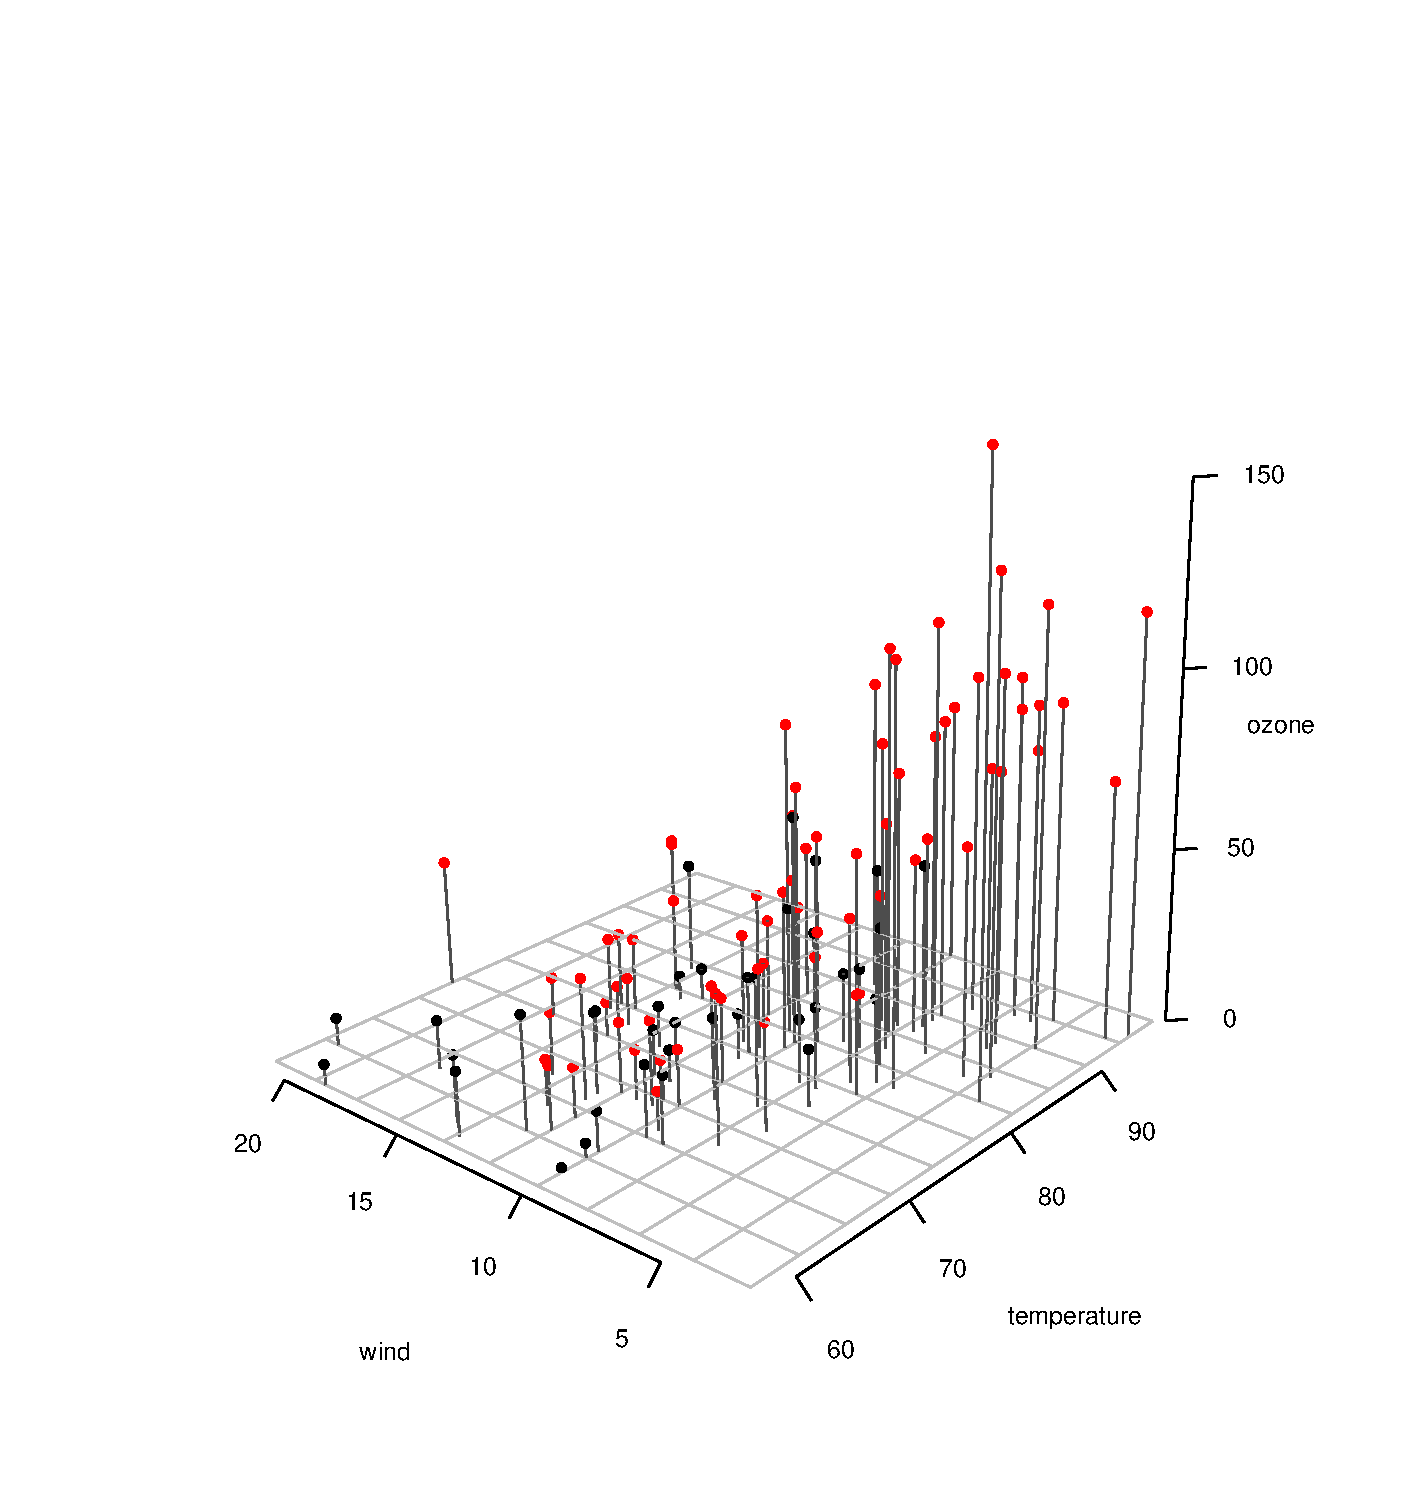
\includegraphics[scale=0.52]{figs/data.pdf}
\caption{The logit of voting preferences over time. Green dots are online polls and blue dots are phone polls.}
\label{data}
\end{center}
\end{figure}
This transformation puts our response variable on the real line, allowing us to model $y_i$ with a normal distribution. Each observation occurred at time $t_i$, which represents the number of days from 1 Sep 2015 (e.g. the first observation is $t_1=4$ as it occurs on 4 Sep 2015). Figure \ref{data} shows the plot of $(t_i, y_i)$ for $i=1,\ldots,n$ but with the x-axis relabeled to show the date corresponding to the $t_i$ value. A quick glance shows difference between the two types of polls.

\subsection{Regression model}

Though we will consider eight models in this paper, they each have the general form
\[ \m{y} \sim N(\m{X} \m{\beta}, \sigma^2 \m{I}) \]
where $\m{y}=(y_1,\ldots,y_n)^\top$. The difference is in the design matrix $\m{X}$. As discussed in the introduction, we wish to explore three aspects of the data: (1) whether there is a linear trend, (2) an effect due to source, and (3) an effect due to poll type. We will build design matrices for each combination, making in total $2^3=8$ models to consider.

Let $\m{t}=(t_1,\ldots,t_n)^\top$ be the vector of days since 1 Sep 2015.

Let $\m{S}$ be the $n\times 6$ binary matrix indicating the source to which the observations belong. That is, for row $i$, the $j$ element is $1$ if observation $i$ belongs to source $j$ and $0$ otherwise. There are six columns in $\m{S}$ since after combining three of the sources, we were left with seven groups. For the design matrix to be full-rank, we must drop one of the columns of $\m{S}$. Here, we choose to drop the Other category, so it will act as a baseline. 

Let $\m{P}$ be the length $n$ binary vector, which element $i$ equal to $1$ is observation $i$ was a phone survey, and $0$ otherwise. This means the online type is our baseline. The eight models each include an intercept term and are constructed by appending combinations of $\m{t}$, $\m{S}$, and $\m{P}$. The design matrix $\m{X}$ for each model is given in Table \ref{models}.
\begin{table}
\caption{Design matrices $\m{X}$ for the eight models}
\centering
\begin{tabular}{ll}
\\ [-5pt]
\hline \hline
Model & $\m{X}$                             \\ \hline
M1    & $(\m{1}_n)$                         \\
M2    & $(\m{1}_n, \m{t})$                  \\
M3    & $(\m{1}_n, \m{S})$                  \\
M4    & $(\m{1}_n, \m{P})$                  \\
M5    & $(\m{1}_n, \m{t}, \m{S})$           \\
M6    & $(\m{1}_n, \m{t}, \m{P})$           \\
M7    & $(\m{1}_n, \m{S}, \m{P})$           \\
M8    & $(\m{1}_n, \m{t}, \m{S}, \m{P})$    \\ \hline\hline
\end{tabular}
\label{models}
\end{table}
By fitting and comparing each model, we can get an idea of whether the components are important in modeling voting preference. The metrics used to compare the models are given in 2.4. Additionally, we may inspect the posterior distribution for $\m{\beta}$ and see which components contain zero in a credible interval.

%\begin{eqnarray*}
%y_i|\mu_i,\sigma^2 &\sim& t_\nu(\mu_i, \sigma^2),~~~~~i=1,\ldots,n \\
%\mu_i|\mu,\tau^2 &\sim& N(\mu, \tau^2),~~~~~i=1,\ldots,n
%\end{eqnarray*}

\subsection{Priors for $\m{\beta}$ and $\sigma^2$}

We use a Zellner's $g$-prior for $\m{\beta}$ and a non-informative prior for $\sigma^2$:
\begin{eqnarray*}
\m{\beta}|\sigma^2 &\sim& N(\m{m}, g\sigma^2(\m{X}^\top\m{X})^{-1}) \\
p(\sigma^2) &\propto& (\sigma^2)^{-1}
\end{eqnarray*}
where $\m{m}$ is chosen as the zero vector and $g$ is fixed at $n$. This specification produces the following posterior full conditionals
\begin{eqnarray*}
\m{\beta}|\sigma^2, \m{y}, \m{X} &\sim& N\left(\frac{1}{g+1}(g\hat{\m{\beta}}-\m{m}), \frac{g\sigma^2}{g+1}(\m{X}^\top\m{X})^{-1}\right) \\
\sigma^2|\m{\beta}, \m{y}, \m{X} &\sim& IG\left(\frac{n}{2}+\frac{p}{n}, \frac{1}{2}(\m{y}-\m{X}\m{\beta})^\top(\m{y}-\m{X}\m{\beta})\right.+ \\
& & ~~~~ ~~~~ ~~~~ \left.\frac{1}{2g}(\m{\beta}-\m{m})^\top(\m{X}^\top\m{X})(\m{\beta}-\m{m})\right)
\end{eqnarray*}
where $\hat{\m{\beta}}=(\m{X}^\top\m{X})^{-1}\m{X}^\top\m{y}$ is the maximum likelihood estimate for $\m{\beta}$ and $p$ is the number of columns of $\m{X}$ (which changes from model to model). Thus we have closed-form full conditionals and we can explore the posterior using Gibbs sampling.

\subsection{Model validation}

We utilize two measures for model fit. The first is a $\chi^2$ test from Johnson (2004) in ``A Bayesian $\chi^2$ Test for Goodness-of-Fit.'' The test is comparable to classical $\chi^2$ goodness-of-fit tests. With this test, we calculate a distribution of $p$-values where high values are in favor of a good model fit. See Johnson (2004) for details.

The second measure is based on leave-one-out cross-validation. We obtain $B$ posterior draws for each model while leaving one observation out, $y_i$. Posterior predictions $y_{j,b}^*$ are then obtained and we compute
\begin{eqnarray*}
p_{j,i}=\frac{1}{B}\sum_{b=1}^B \mathds{1}(y_{j,b}^* \leq y_i),~~~~~j=1,\ldots,8
\end{eqnarray*}
Distribution theory requires that $p_{j,\cdot}$ be uniformly distributed for the model to be appropriate. The Kolmogorov-Smirnov (K-S) test is used to determine whether $p_{j,\cdot}$ is uniform.

Graphically, a kernel density plot of the posterior predictive distribution against the data can provide a quick assessment for the model fit.

\subsection{Model comparison}

To compare the models, we use two measures. The deviance information criterion (DIC) is defined as
\begin{eqnarray*}
DIC=\bar{D}(\theta)+\widehat{\mathrm{var}}(D(\theta))/2
\end{eqnarray*}
where $D(\theta)=-2\log p(\m{y}|\theta)$, $\bar{D}(\theta)$ is the average of $D(\theta)$ over all posterior samples $\theta$ and $\widehat{\mathrm{var}}(D(\theta))$ is the sample variance of $D(\theta)$. DIC measures goodness-of-fit and penalizes model complexity; a lower DIC is preferred.

The second measure is the posterior predictive loss (PPL) which is similar in nature to DIC. It is computed by
\begin{eqnarray*}
PPL=G+P=\sum_{i=1}^n(y_i-\mu_i^*)^2 + \sum_{i=1}\sigma_i^*
\end{eqnarray*}
where $\mu_i^*$ and $\sigma_i^*$ are the mean and variance of the posterior prediction for observation $i$. We put more faith in DIC over PPL, since as model complexity grows, PPL is not punished as much as it should.

\section{Results}

In all subsequent analyses, we retain $B=10000$ posterior samples after a burn-in period. We first analyze whether the eight models are adequate fits to the data. We obtain a distribution of $p$-values (based on a $\chi^2$ test) for each model. These are shown in Figure \ref{gof}. Small $p$-values give evidence that the model is inadequate. The only two models that seem to be inadequate are M1 and M2, the intercept-only model and the intercept and linear trend model, respectively.
\begin{figure}
\centering
\includegraphics[scale=0.55]{figs/gof.pdf}
\caption{Distribution of $p$-values for the eight models (identified by color) for the Bayesian goodness-of-fit test.}
\label{gof}
\end{figure}

Leave-one-out cross-validation shows similar findings (see Figure \ref{loo}). Distributions that are uniform give evidence that the model fits. A visual inspection suggests that, again, only M1 and M2 are questionable. However, the K-S test resulted in $p$-values greater than $0.19$ in every case. Hence, there is some evidence that suggests M1 and M2 are inadequate, but no evidence for M3-M8 to be poor fits. Figure \ref{obsfit} shows a plot of observed versus fitted values (on the logit scale) and Figure \ref{pred_time} shows posterior predictions (on the original scale) across time, both for M8. 
\begin{figure}
\centering
\includegraphics[scale=0.55]{figs/loo.pdf}
\caption{Distributions of the CDF evaluated at each observation based on leave-one-out cross-validation.}
\label{loo}
\end{figure}

We now address the main questions: is there a time trend? is there an effect due to polling source? and is there an effect due to poll type? We answer these by comparing the eight models. M8 includes all terms ($\m{t}$, $\m{S}$, $\m{P}$ as described in 2.1) and is considered the full model. If we remove some of these terms, do we still have a sufficient model?

\begin{table}
\caption{Model comparison quantities}
\centering
\begin{tabular}{lrrrr}
\\ [-5pt]
\hline\hline
   & DIC     & G    & P    & G+P  \\ \hline
M1 &  -97.47 & 2.12 & 2.20 & 4.32 \\
M2 &  -96.92 & 2.10 & 2.18 & 4.28 \\
M3 & -158.06 & 1.02 & 1.14 & 2.17 \\
M4 & -180.62 & 0.90 & 0.96 & 1.87 \\
M5 & -158.32 & 1.00 & 1.13 & 2.13 \\
M6 & -195.31 & 0.76 & 0.82 & 1.59 \\
M7 & -182.75 & 0.78 & 0.88 & 1.67 \\
M8 & -199.31 & 0.65 & 0.74 & 1.39 \\ \hline\hline
\end{tabular}
\label{dic}
\end{table}

Table \ref{dic} presents the DIC and PPL for each model. M8 does the best under both criteria. M6 (removal of the source effect) is not far behind. This would suggest that there may be no source effect. But removing the time trend (M7) or the polling type (M5) from the full model has a much more dramatic change in DIC, suggesting that both effects are real. In addition,under M8 the posterior distributions for the elements in $\m{\beta}$ corresponding to the source effects all have zero in their 95\% HPD (Figure \ref{post}).

\begin{figure*}
\centering
\includegraphics[scale=0.51]{figs/pred_time.pdf}
\caption{Posterior predictions for M8, back-transformed to the original scale. The black is the data. The middle blue line is the predictive mean and the outer blue lines are equal-tailed 95\% posterior intervals.}
\label{pred_time}
\end{figure*}

Given these results, M6 would seem to perform just as well as M8 and perhaps better since it would be less prone to overfitting. This is to say there is a linear time trend, which is steadily increasing in favor of leaving the EU, and that the type of poll has a noticeable impact on polling results with phone surveys showing preferences toward remaning.

\begin{figure}
\centering
\includegraphics[scale=0.53]{figs/pred_obsfit.pdf}
\caption{Plot for observed versus fitted for M8. The dots are mean predictions and the lines are equal-tailed 95\% predictive intervals. The black line is the line $y=x$.}
\label{obsfit}
\end{figure}


\section{Discussion}

We have explored the recent UK polls on voter preferences regarding the EU referendum. There is evidence that opinions have changed over time and that we are seeing a steady increase toward leaving the EU. Though, depending on the type of survey (whether online or phone) we are seeing different polling results. This is likely due in large part because of the accessibility of online surveys and the type of people responding to these polls.

Our regression models provide adequate fits to the data, but some perform better than others. A full model accounting for time, source, and poll type does well. But a model with only time and poll type performs nearly on the same level. In the end, the real voting takes place in a month and many of those people making bets on the outcome are going to lose a lot of money.

\begin{figure}
\centering
\includegraphics[scale=0.35]{figs/post.pdf}
\caption{Marginal posterior distributions for $\m{\beta}$ for M8. The shaded regions are the 95\% HPD intervals and the red vertical lines mark $x=0$.}
\label{post}
\end{figure}

\end{document}
